\section{Experiment \& Result} \label{section:experiment_result}

In this section, first, we present our experiment result on Oxford 5K Building Dataset to prove that our BoW implementation can achieve good enough performance on standard benchmark. The experiment shows that our version of BoW achieves the mean average precision of 0.844 on Oxford 5K Building Dataset with nearly one second average time for each query. This dataset was constructed by Philbin et al. in 2007 \cite{2}. It consists of 5,062 images of resolution $1024 \times 768$ belongs to 11 different Oxford buildings. Images for each building are collected from Flickr by searching using text queries. Along with the dataset, there are also 55 queries along with their ground-truth, 5 for each landmark. The ground truth of 55 queries are manually constructed. For each query, images are classified into 4 groups: (1) \textit{Good}: the building appears apparently, (2) \textit{OK}: more than 25\% of the building is present, (3) \textit{Bad}: the building is not shown up, and (4) \textit{Junk}: less than 25\% of the building is captured. The reason why the authors use this dataset is because of its popularity, it is used by many previous works in this field. Thus, we can easily compare our systems with those previous works.

Secondly, we also present and illustrate several typical scenarios of our automatic annotation system with the dataset consisting of our personal photos taken from Facebook. This dataset includes 5 different classes corresponding with 5 social events that are personally annotated. There are 2 classes that share a common annotation. Photos in each class share some particular attributes such as background, mascots, logos. As a result, whenever users create or edit the annotation of these common objects, other photos in the same class can also be tagged similarly thanks to theses mutual attributes. The details of these 5 classes in the dataset are described below:

\begin{enumerate}

\item \#APCS\_Party: Photos taken at a party of my university. Photos in this class contain nearly the same group of people and have similar background and decoration on the stage.
\item \#First\_time\_in\_Singapore: These photos are taken at the Merlion in Singapore. They all contain the merlion statue.
\item \#Hoi\_An\_with\_family: These photos are taken at Hoi An town in Vietnam with one of the authors' family. The people appearing in them and the background are their common attributes.
\item \#My\_favoriate\_competition: These are taken at multiple times I have taken part in the ACM-ICPC, a really famous collegiate programming competition. The mutual characteristic of these photos is the logo of the competition.
\item \#My\_first\_regional: These photos are taken at my ICPC regional contest in Phuket, Thailand. The photos all accommodate the mascot of the competition.

\end{enumerate}

\begin{figure}
    \centering
    \begin{tabular}{ccc}
		\subfloat{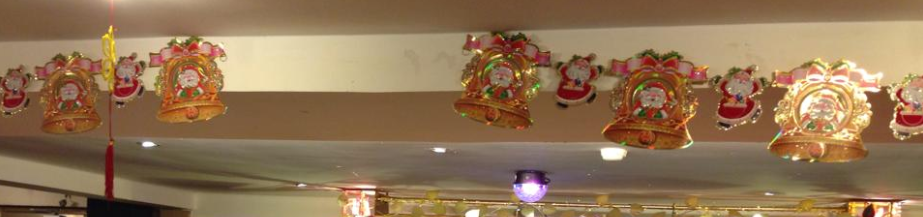
\includegraphics[width = 1.3in]{APCS_check_0_query.png}} &
		\subfloat{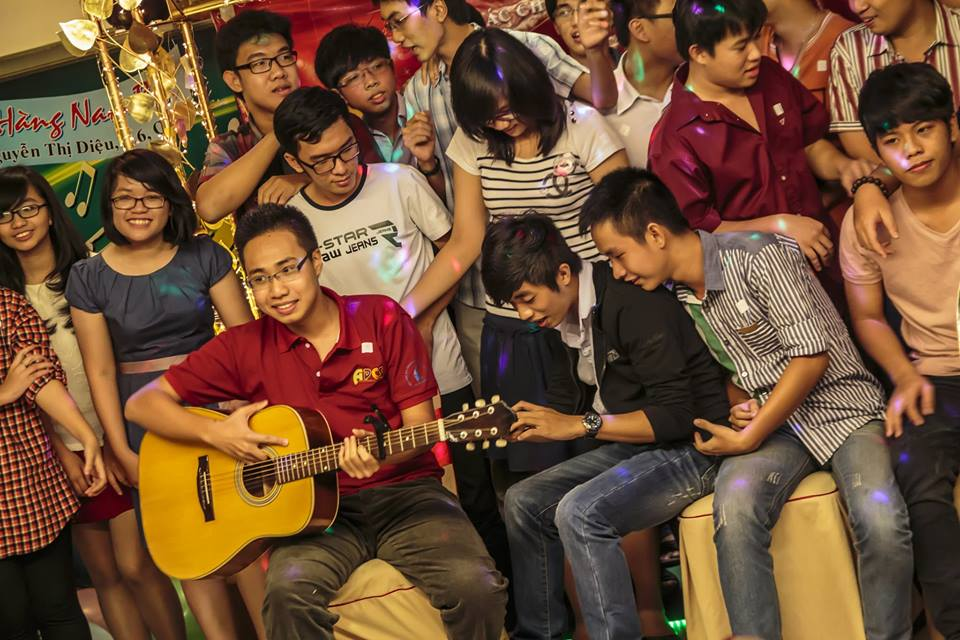
\includegraphics[width = 1.3in]{APCS_2.jpg}} &
		\subfloat{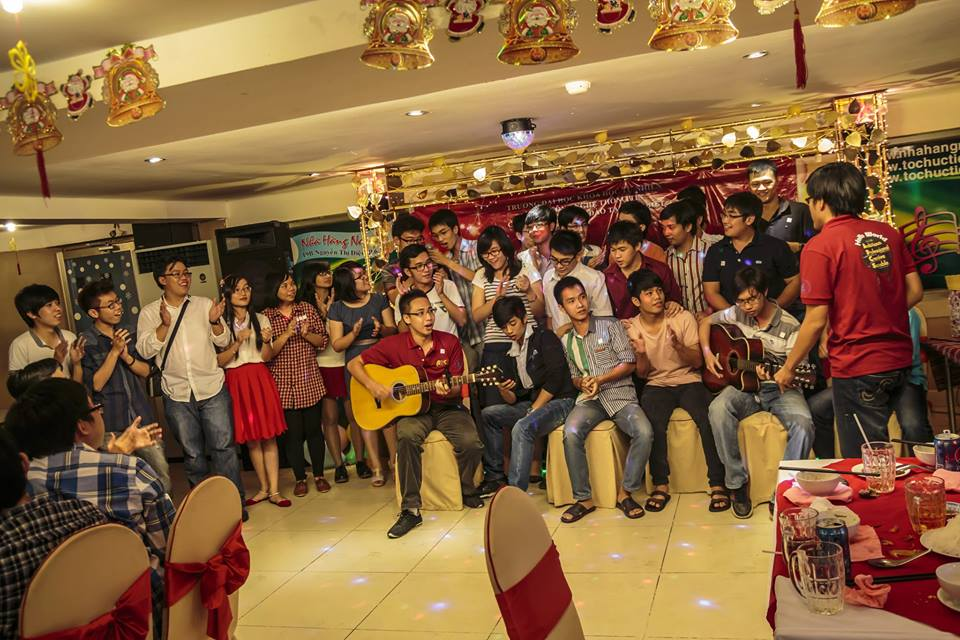
\includegraphics[width = 1.3in]{APCS_3.jpg}} \\
		& \#APCS\_Party & \\
		
		\subfloat{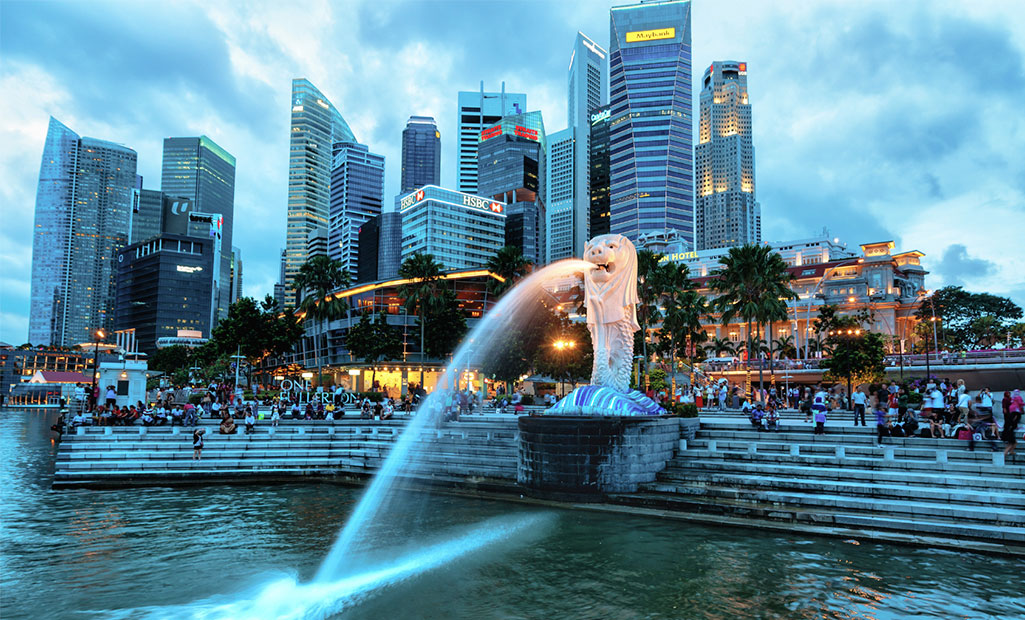
\includegraphics[width = 1.3in]{Merlion_check_0_query.jpg}} &
		\subfloat{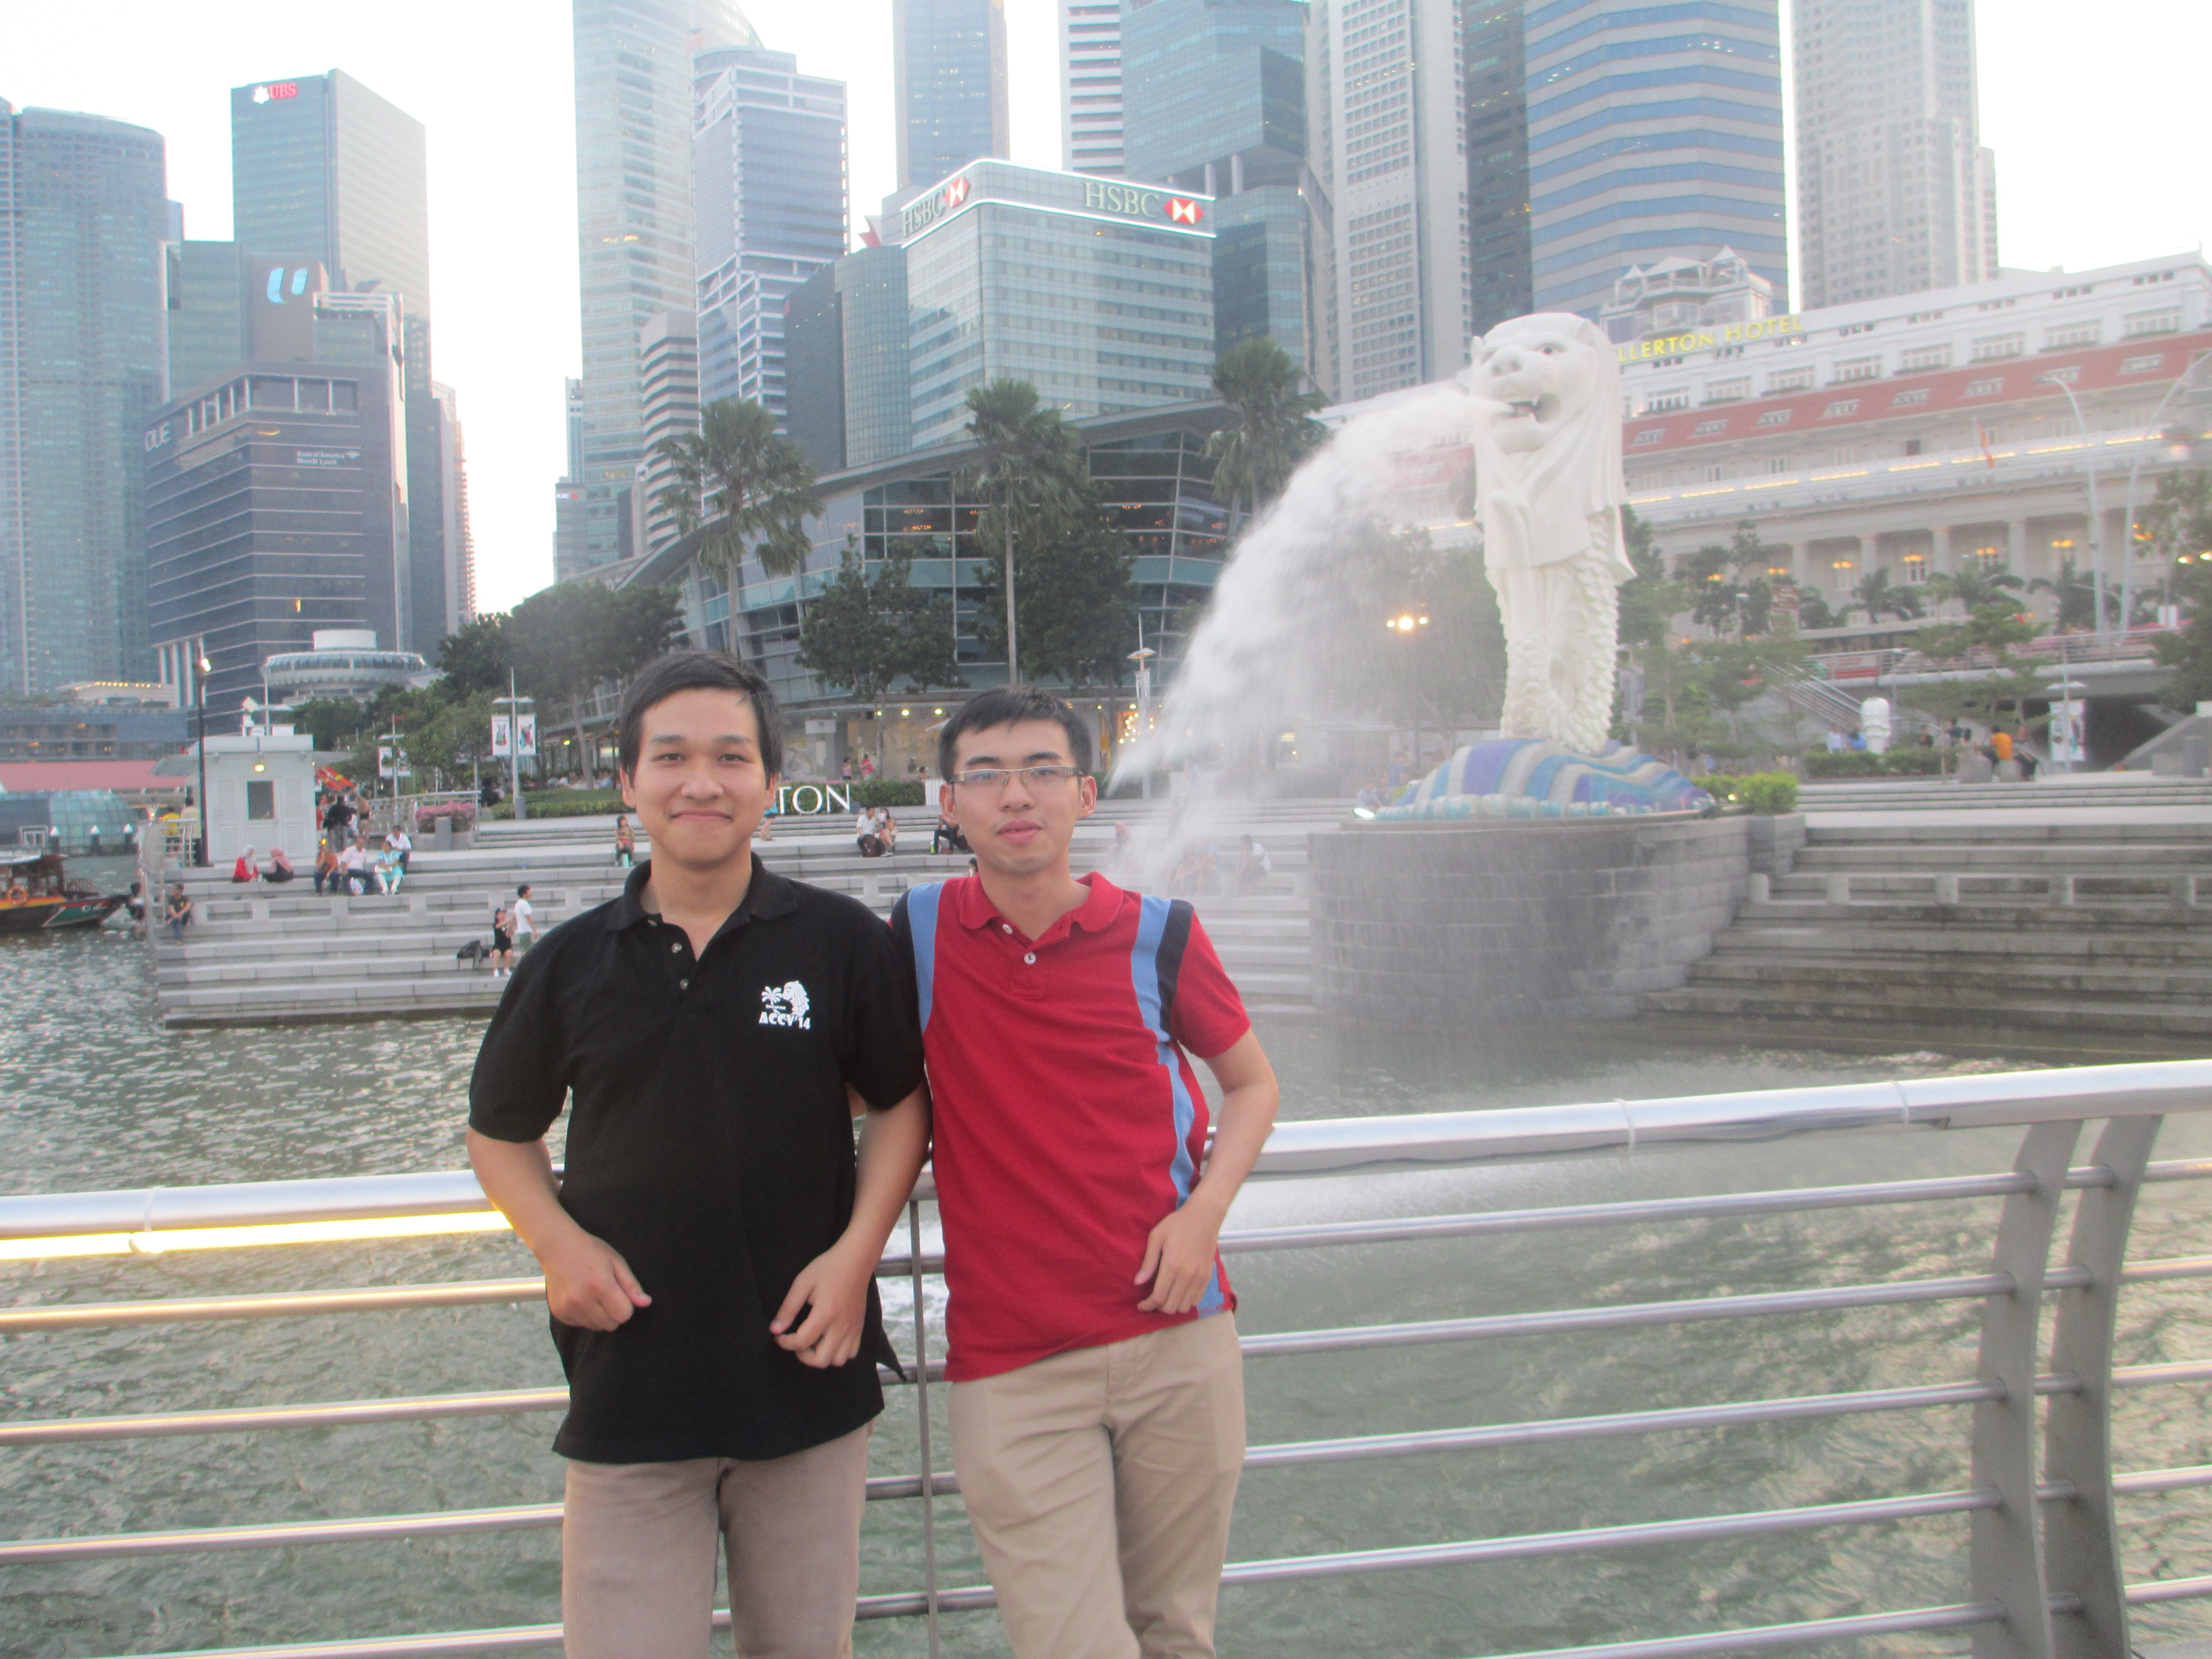
\includegraphics[width = 1.3in]{singapore_3.jpg}} &
		\subfloat{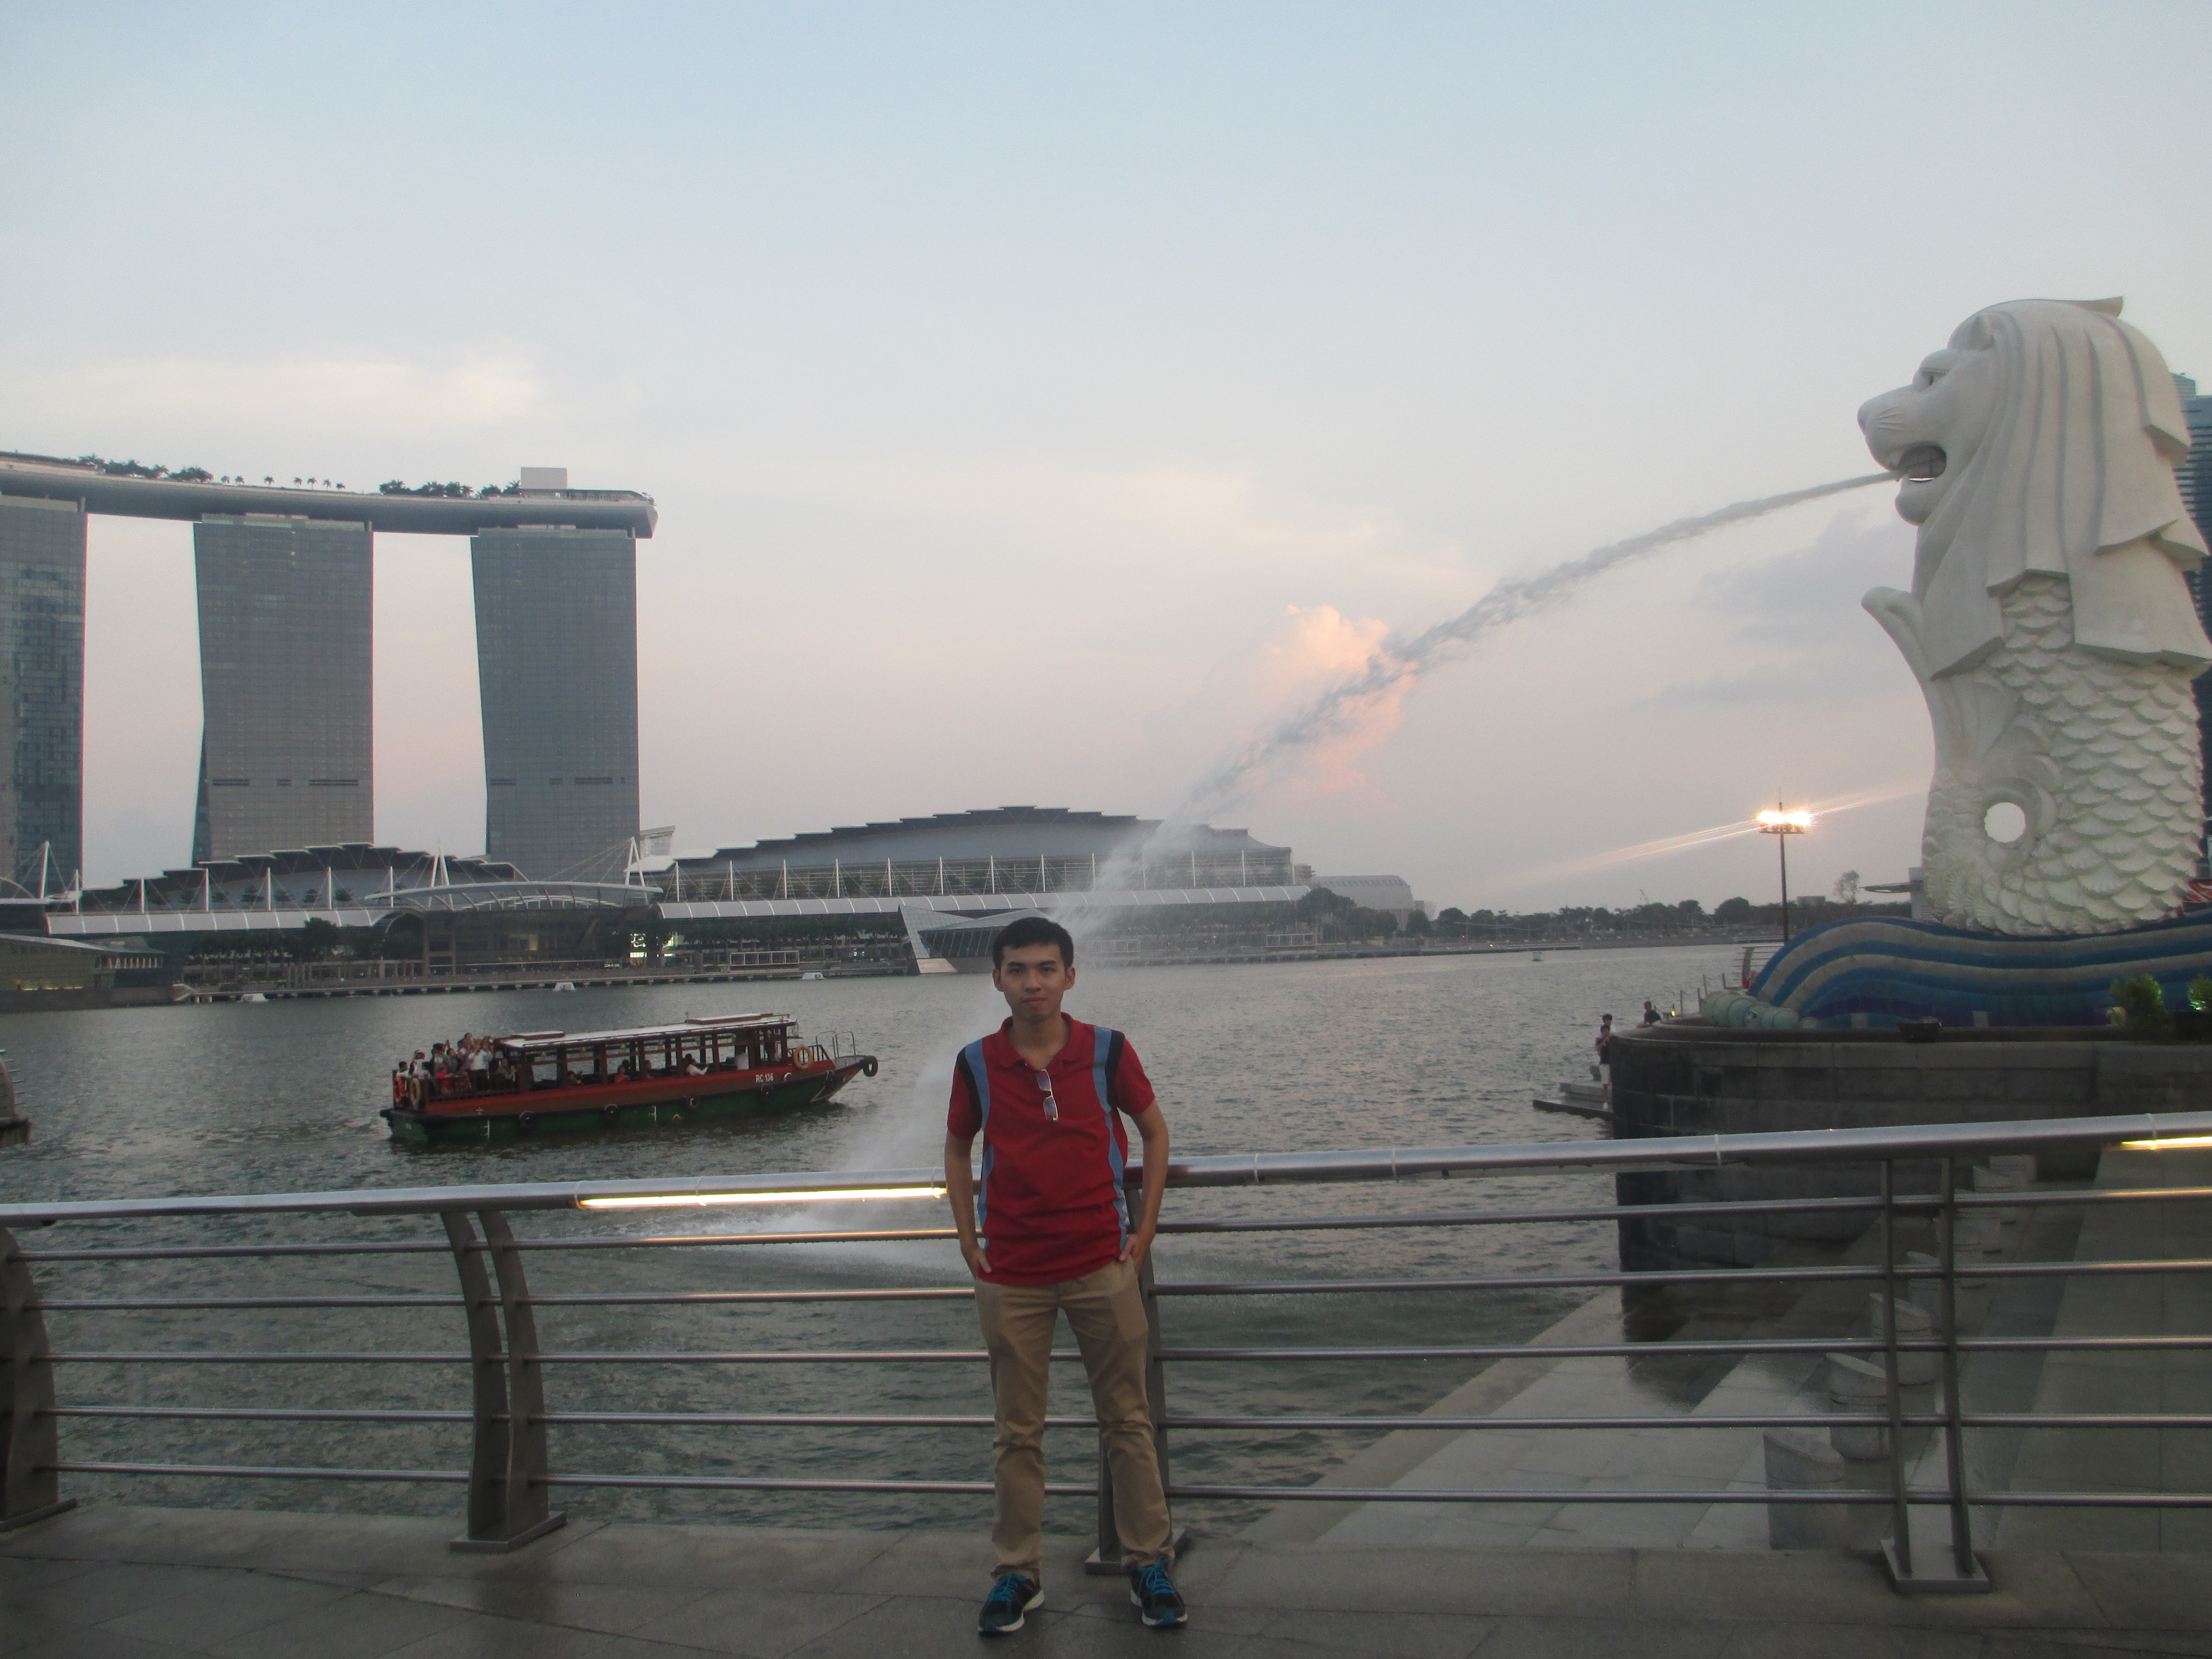
\includegraphics[width = 1.3in]{singapore_4.jpg}} \\
		& \#First\_time\_in\_Singapore & \\
		
		\subfloat{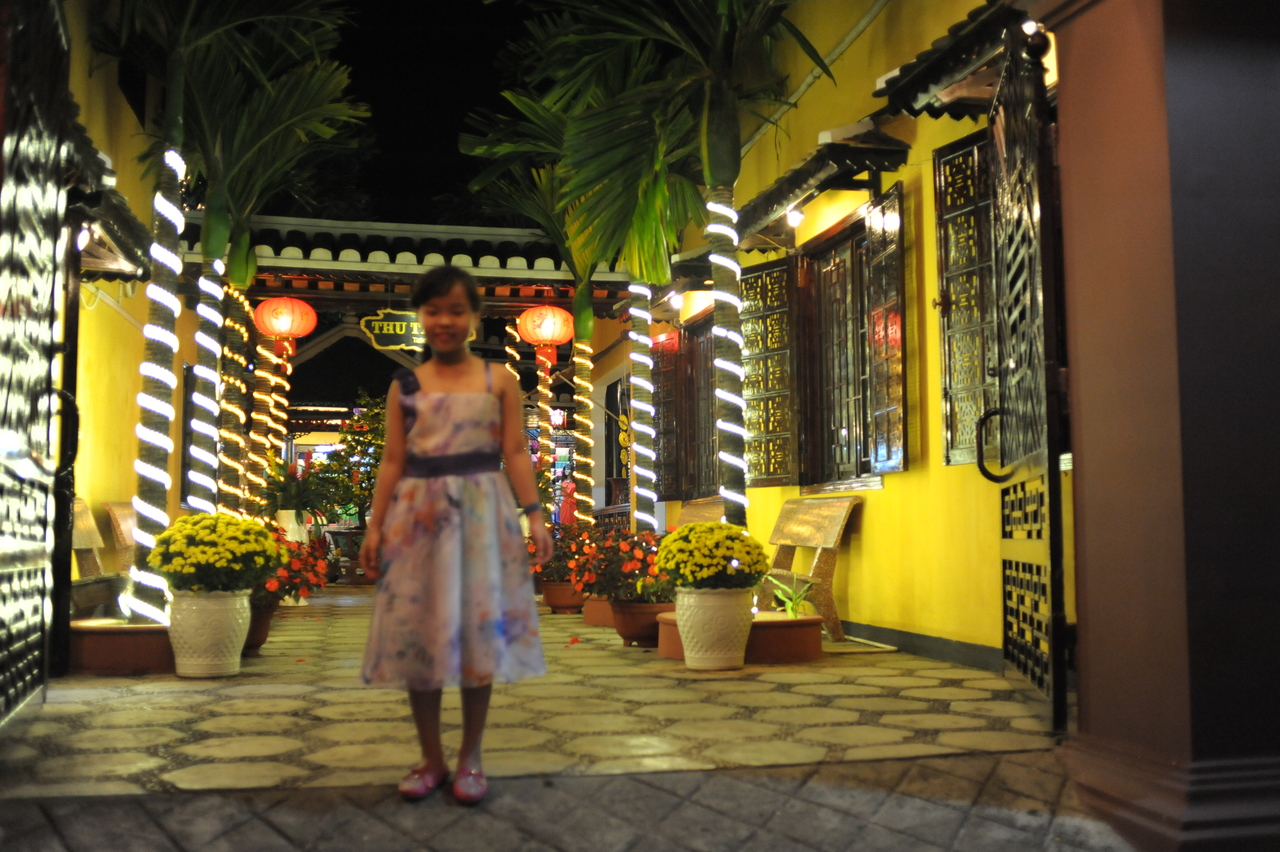
\includegraphics[width = 1.3in]{Hoian_check_0_query.jpg}} &
		\subfloat{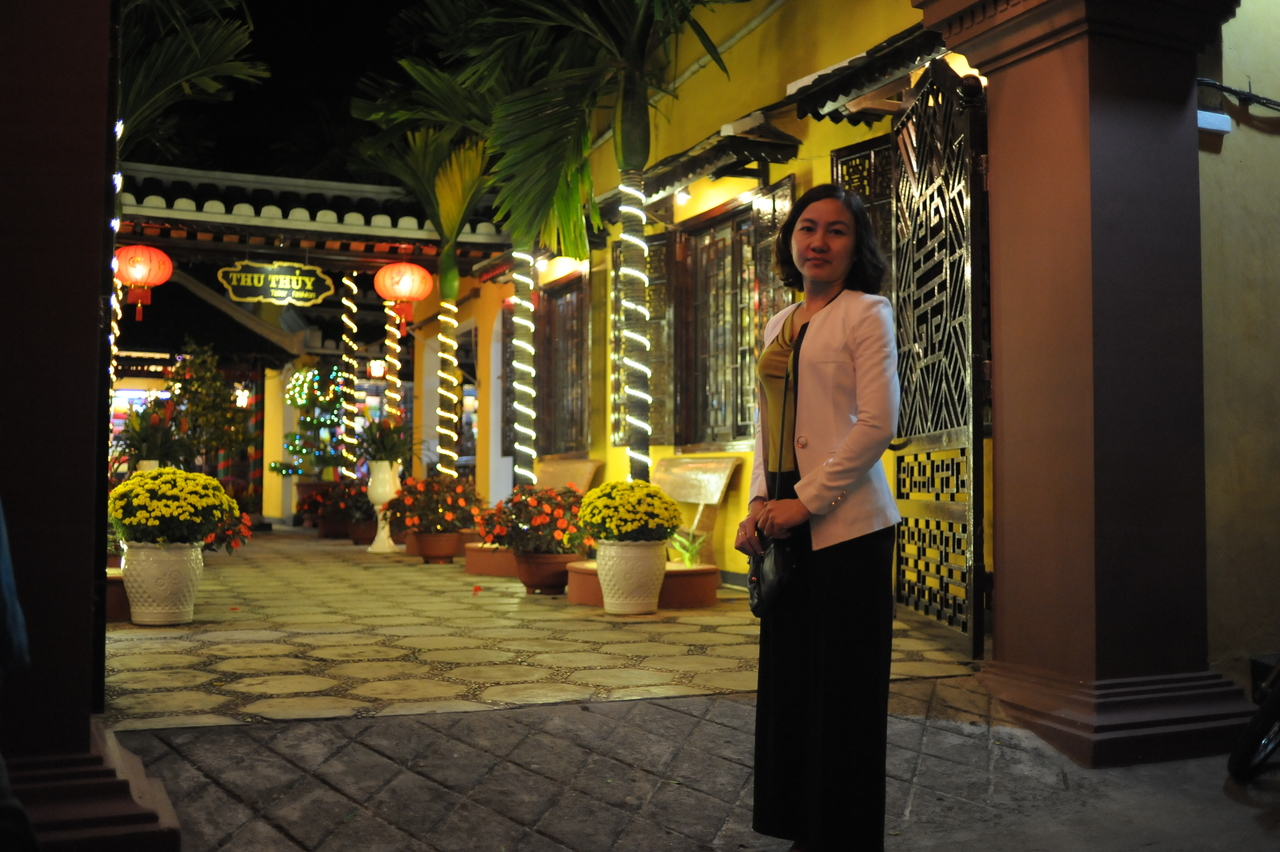
\includegraphics[width = 1.3in]{hoian_7.jpg}} &
		\subfloat{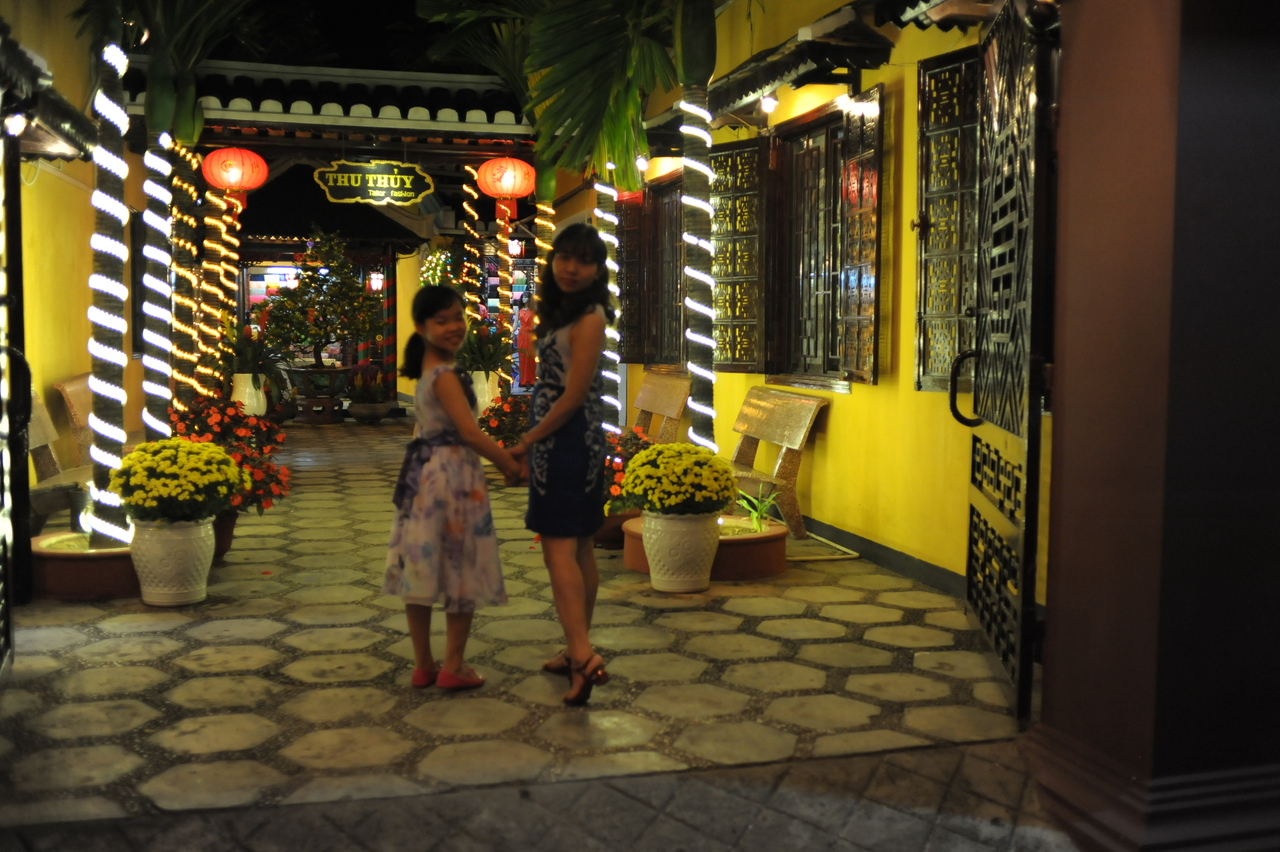
\includegraphics[width = 1.3in]{hoian_11.jpg}} \\
		& \#Hoi\_An\_with\_family & \\
		
		\subfloat{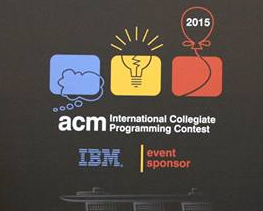
\includegraphics[width = 1.3in]{ACM_check_0_query.png}} &
		\subfloat{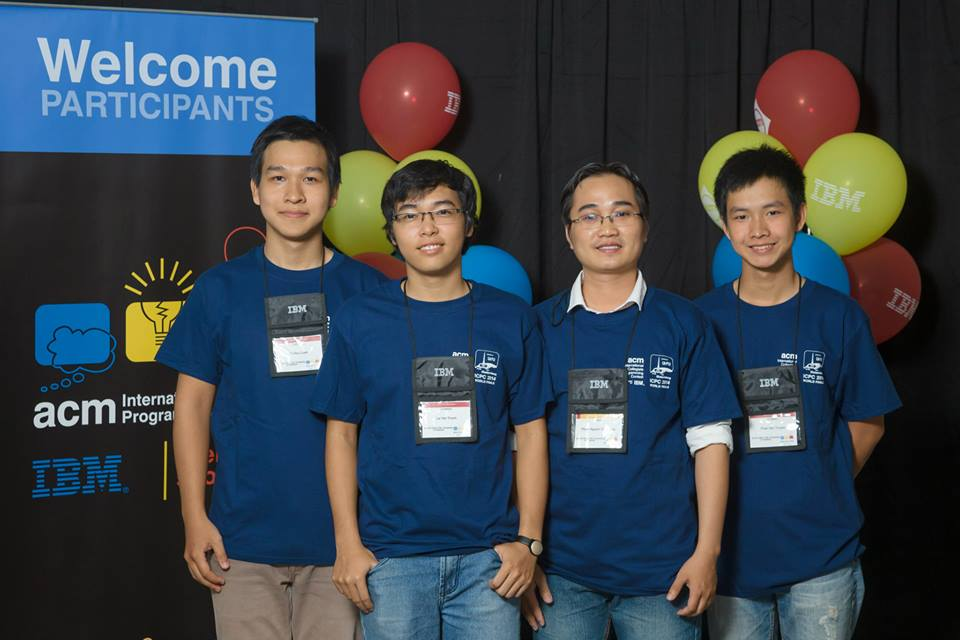
\includegraphics[width = 1.3in]{icpc_1.jpg}} &
		\subfloat{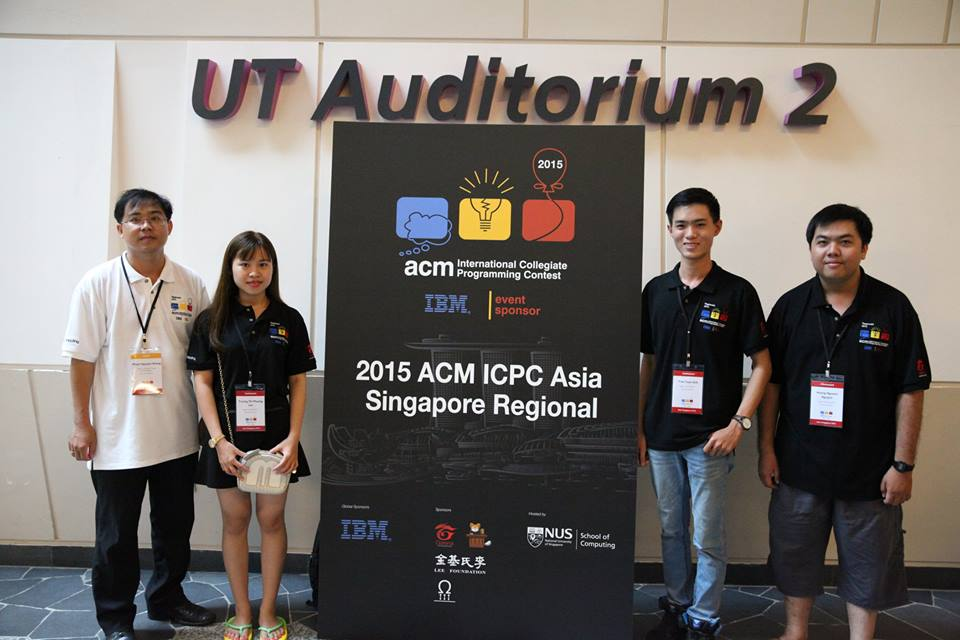
\includegraphics[width = 1.3in]{icpc_7.jpg}}	\\
		& \#My\_favorite\_competition & \\
		
		\subfloat{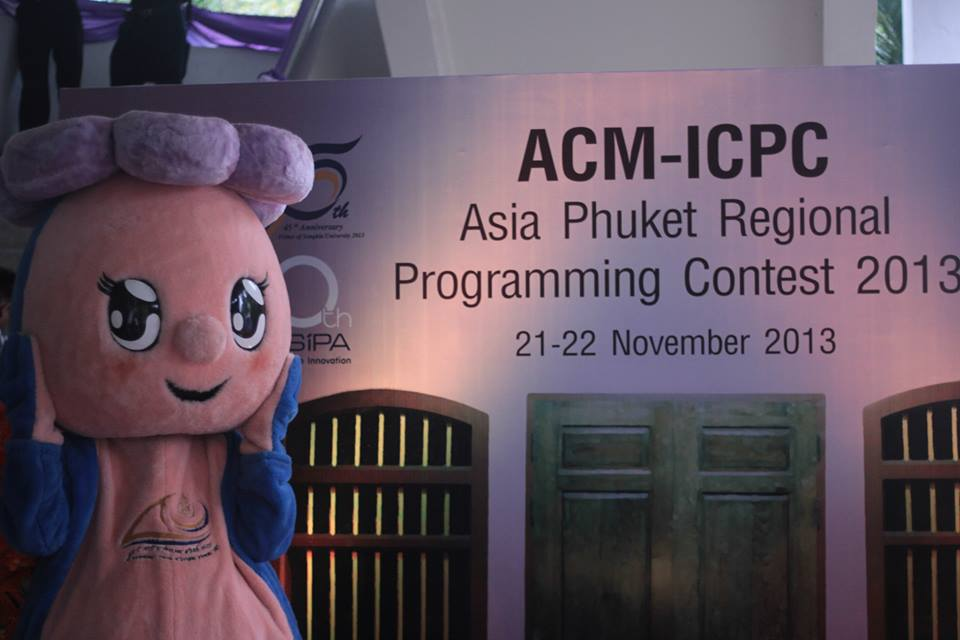
\includegraphics[width = 1.3in]{thailand_check_0_query.jpg}} &
		\subfloat{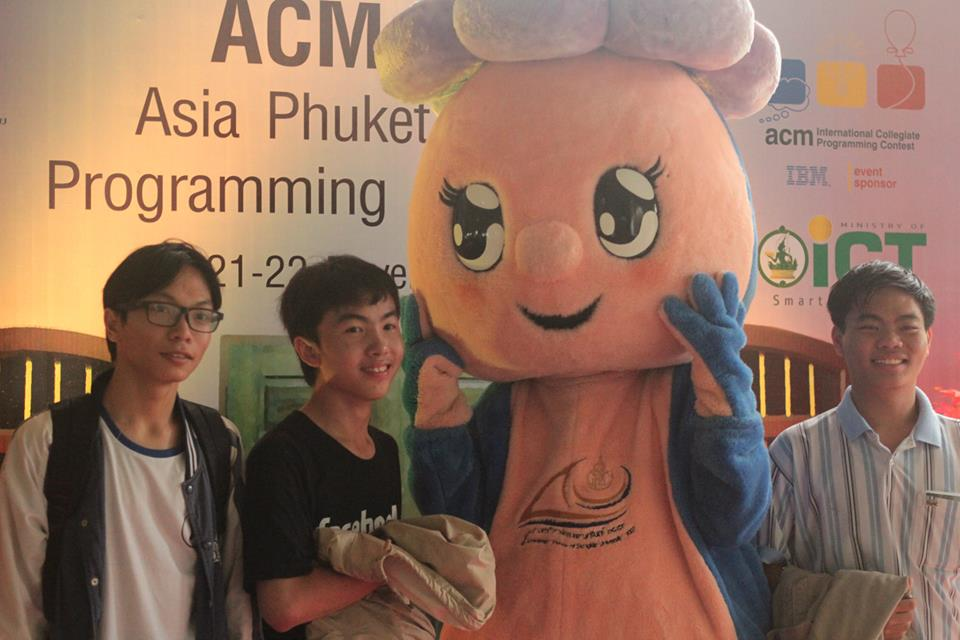
\includegraphics[width = 1.3in]{thailand_3.jpg}} &
		\subfloat{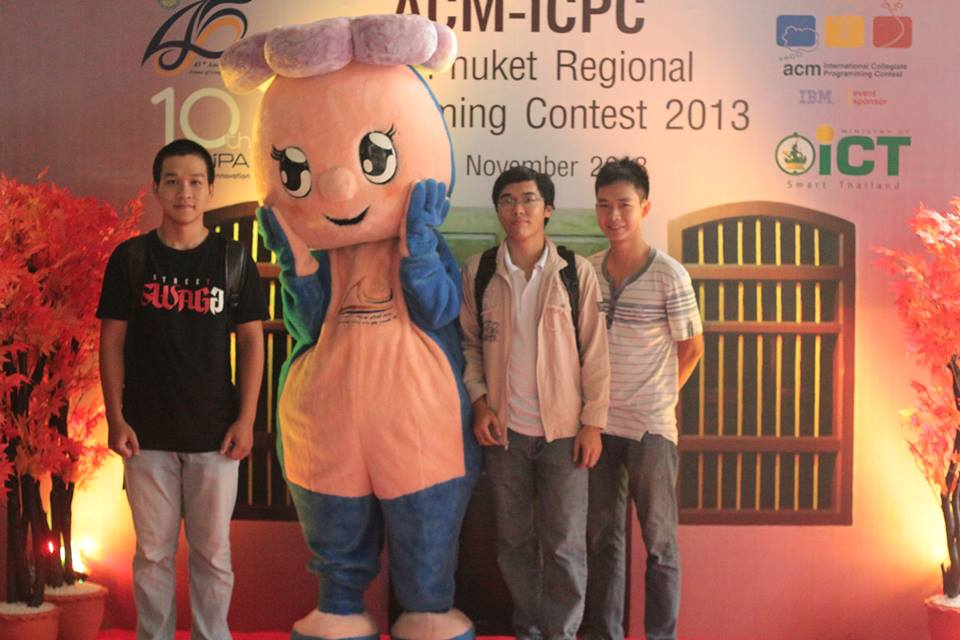
\includegraphics[width = 1.3in]{thailand_4.jpg}} \\
		& \#My\_first\_Regional & \\
		
		(a) & (b) & (c) \\
	\end{tabular}
    \caption{Our personal dataset. Column (a) shows 5 queries of 5 classes in the dataset. Column (b) and (c) are some examples in the returned result of the queries.}
    \label{fig:personal_dataset}
\end{figure}

We then performed experiment on 5 different queries corresponding to 5 different classes. These queries and some sample result are given in Fig. \ref{fig:personal_dataset}. In the experiment, each query also takes our system nearly one second on average and the mean average precision over 5 queries is 0.749. The detail result is shown in table \ref{tab:detail_result}.

\begin{table}[h!]
  \centering
  
  \begin{tabular}{cccccc}
    \toprule
    APCS query & Singapore query & Thailand query & ACMlogo query & HoiAn query & \textbf{mAP} \\
    \midrule
    0.690 & 0.775 & 0.798 & 0.754 & 0.728 & \textbf{0.749} \\
    \bottomrule
  \end{tabular}
  \caption{Experiment on personal dataset}
  \label{tab:detail_result}
\end{table}